\documentclass[10pt]{article}
 
\usepackage[margin=1in]{geometry} 
\usepackage{amsmath,amsthm,amssymb, graphicx, multicol, array}
\usepackage{mathtools}
\usepackage{booktabs}
\usepackage{stata/stata}
\usepackage{wrapfig}

\graphicspath{ {images/} }

\newcommand\iid{\stackrel{\mathclap{iid}}{\sim}}
\newcommand\asym{\stackrel{\mathclap{a}}{\sim}}
\newcommand\convprob{\xrightarrow{p}}
\newcommand\convdist{\xrightarrow{d}}
\newcommand{\N}{\mathbb{N}}
\newcommand{\Z}{\mathbb{Z}}
\newcommand{\E}{\text{E}}
\newcommand{\V}{\text{Var}}
\newcommand{\Av}{\text{Avar}}
\newcommand{\se}{\text{se}}
\newcommand{\corr}{\text{Corr}}
\newcommand{\cov}{\text{Cov}}
\newcommand{\norm}{\text{Normal}}
\newcommand{\indep}{\perp \!\!\! \perp}

 
\newenvironment{problem}[2][Problem]{\begin{trivlist}
\item[\hskip \labelsep {\bfseries #1}\hskip \labelsep {\bfseries #2.}]}{\end{trivlist}}

\begin{document}
 
\title{Homework 3}
\author{ECON 7023: Econometrics II\\
Maghfira Ramadhani\\
February 21, 2022}
\date{Spring 2023}
\maketitle

\section*{Chapter 5}
\subsection*{Problem 5.4}
Use the data in CARD.RAW for this problem
\begin{enumerate}
\item[a.] Estimate a $\log(wage)$ equation by OLS with $educ, exper, exper^2, black, south, smsa, reg661$ through $reg668$, and $smsa66$ as explanatory variables. Compare your results with Table 2, Column (2) in Card (1995).
\\ Answer:
\begin{figure}[h]
    \caption{Result from Card (1995)} \label{Fig3.1}
    \centering
    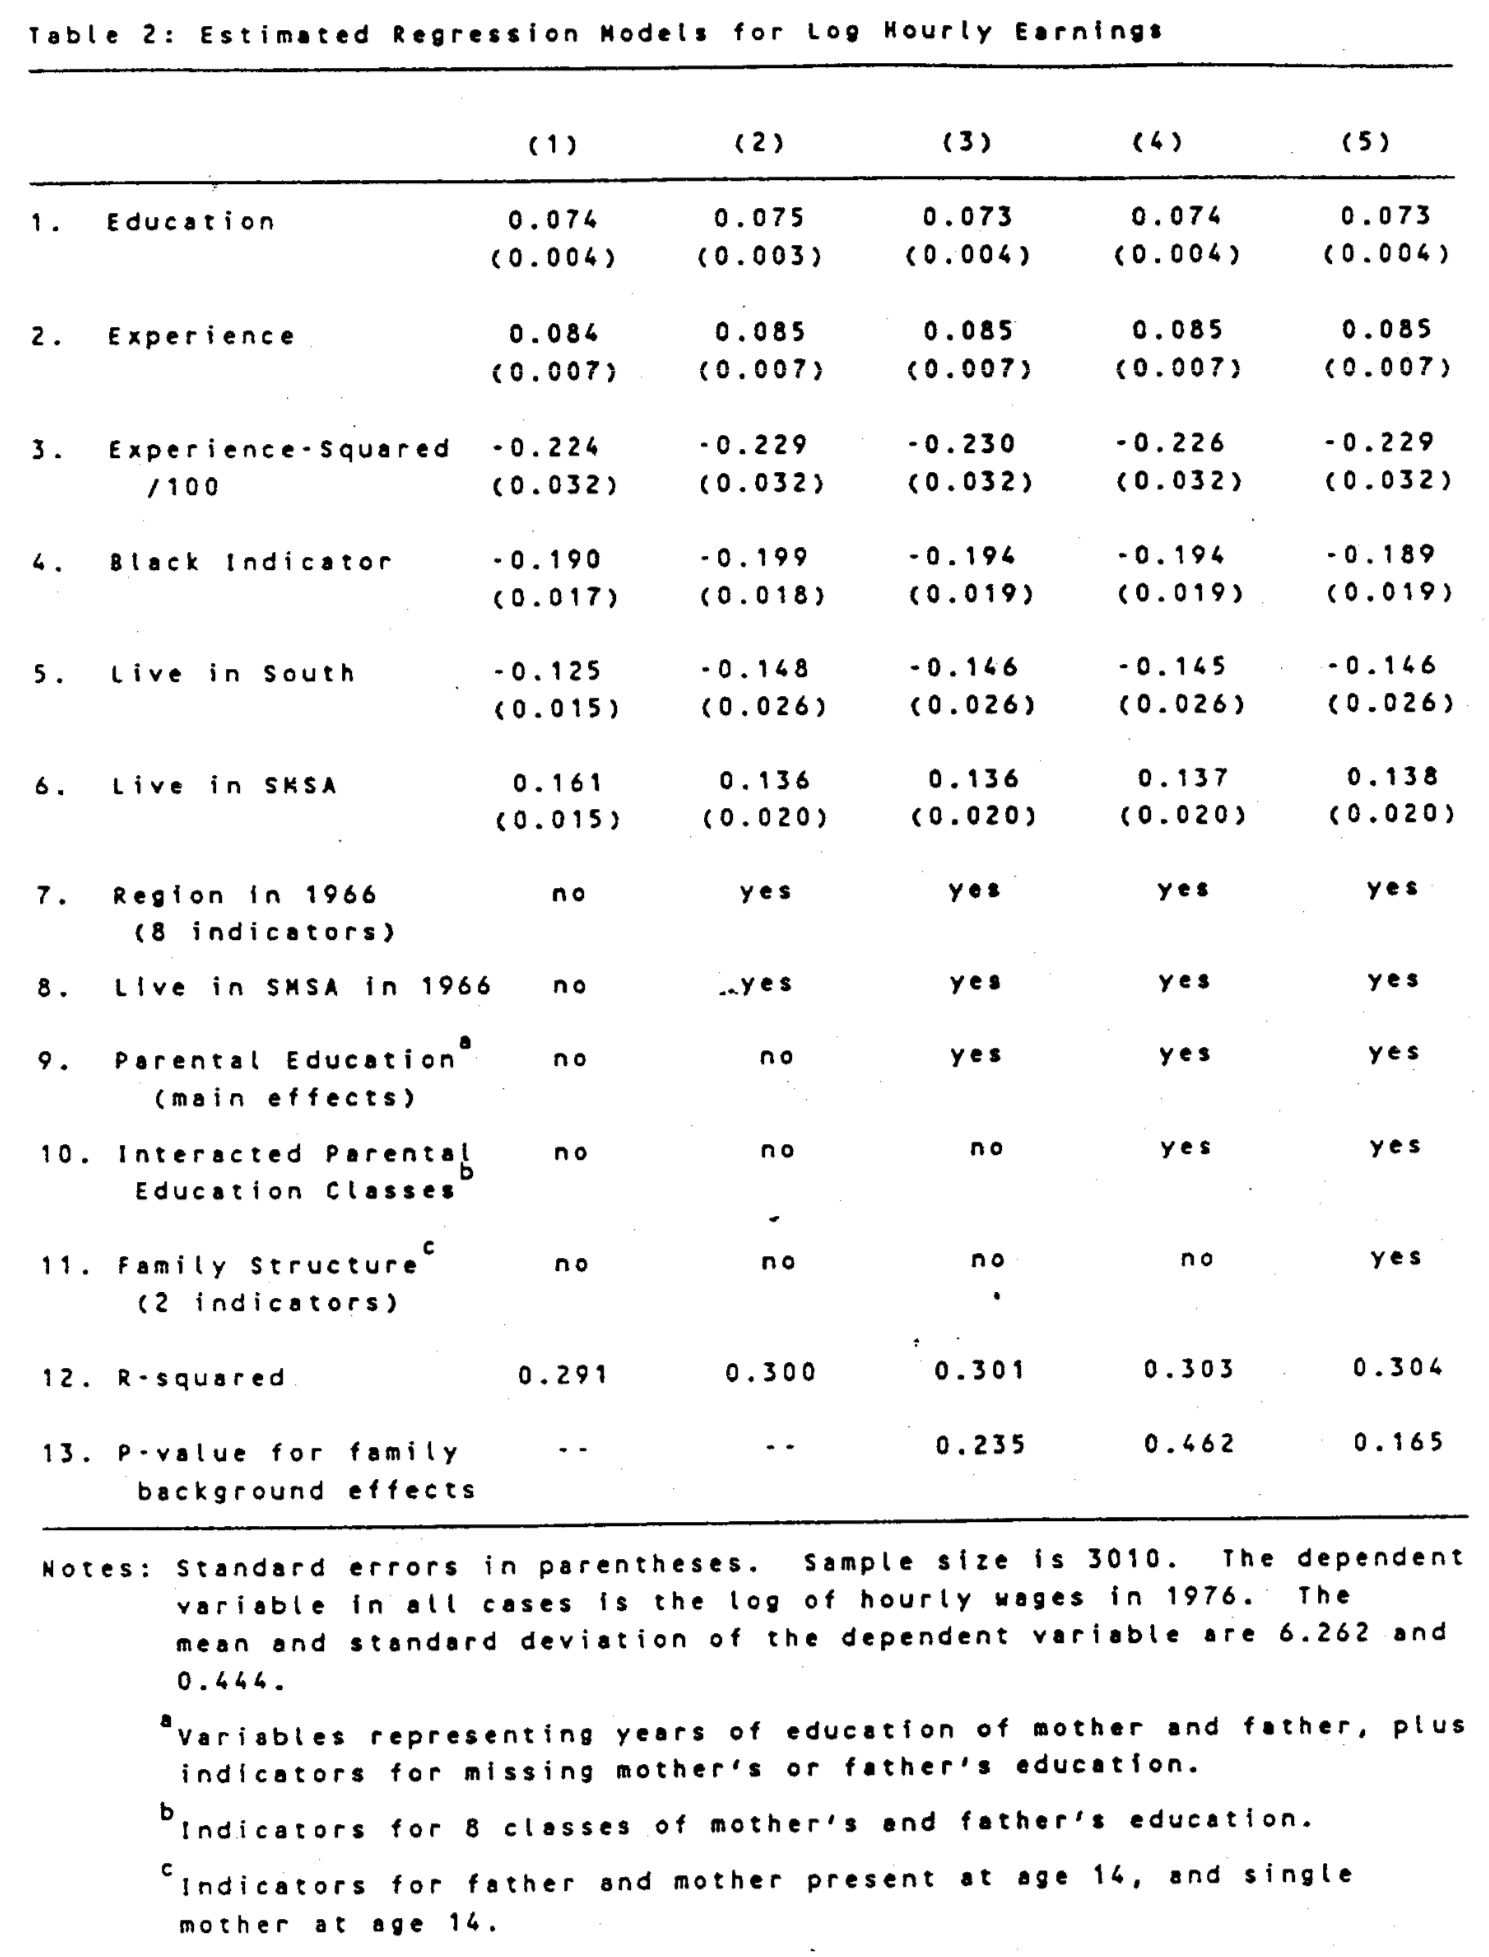
\includegraphics[scale=0.23]{table2.png}
\end{figure}
\\
From Figure \ref{Fig3.1}, we know that the result in Column (2) the return to education is 7.5\% with standard error of 0.03\% and is statistically significant. Comparing to the result that we have in Table 1 from estimating $\log(wage)$ by OLS with $educ, exper, exper^2, black, south, smsa, reg661$ through $reg668$, and $smsa66$ as explanatory variables, we also get 7.5\% return of education with standard error of 0.03\% and is statistically significant. Surprisingly, we get the same coefficient and standard error with those in Card (1995) even though the model specifications are different.
\begin{table}[htbp]\centering
\def\sym#1{\ifmmode^{#1}\else\(^{#1}\)\fi}
\caption{Regression result for Problem 5.4.a.}
\begin{tabular}{l*{1}{c}}
\toprule
                    &\multicolumn{1}{c}{(1)}         \\
\midrule
years of schooling, 1976&       0.075\sym{***}\\
                    &     (0.003)         \\
\addlinespace
age - educ - 6      &       0.085\sym{***}\\
                    &     (0.007)         \\
\addlinespace
exper^2             &      -0.002\sym{***}\\
                    &     (0.000)         \\
\addlinespace
=1 if black         &      -0.199\sym{***}\\
                    &     (0.018)         \\
\addlinespace
=1 if in south, 1976&      -0.148\sym{***}\\
                    &     (0.026)         \\
\addlinespace
=1 in in SMSA, 1976 &       0.136\sym{***}\\
                    &     (0.020)         \\
\addlinespace
regional dummy, 1966&      -0.119\sym{***}\\
                    &     (0.039)         \\
\addlinespace
reg662              &      -0.022         \\
                    &     (0.028)         \\
\addlinespace
reg663              &       0.026         \\
                    &     (0.027)         \\
\addlinespace
reg664              &      -0.063\sym{*}  \\
                    &     (0.036)         \\
\addlinespace
reg665              &       0.009         \\
                    &     (0.036)         \\
\addlinespace
reg666              &       0.022         \\
                    &     (0.040)         \\
\addlinespace
reg667              &      -0.001         \\
                    &     (0.039)         \\
\addlinespace
reg668              &      -0.175\sym{***}\\
                    &     (0.046)         \\
\addlinespace
=1 if in SMSA, 1966 &       0.026         \\
                    &     (0.019)         \\
\addlinespace
Constant            &       4.739\sym{***}\\
                    &     (0.072)         \\
\midrule
Observations        &        3010         \\
\bottomrule
\multicolumn{2}{l}{\footnotesize Standard errors in parentheses}\\
\multicolumn{2}{l}{\footnotesize Data: CARD.DTA}\\
\multicolumn{2}{l}{\footnotesize Wooldridge (2011)}\\
\multicolumn{2}{l}{\footnotesize \sym{*} \(p<0.10\), \sym{**} \(p<0.05\), \sym{***} \(p<0.01\)}\\
\end{tabular}
\end{table}


\item[b.] Estimate a reduced form equation for $educ$ containing all explanatory variables from part a and the dummy variable $nearc4.$ Do $educ$ and $nearc4$ have a practically and statistically significant partial correlation? (See also Table 3, Column (1) in Card (1995).)
\\ Answer:
\begin{figure}[h]
    \caption{Result from Card (1995)} \label{Fig3.2}
    \centering
    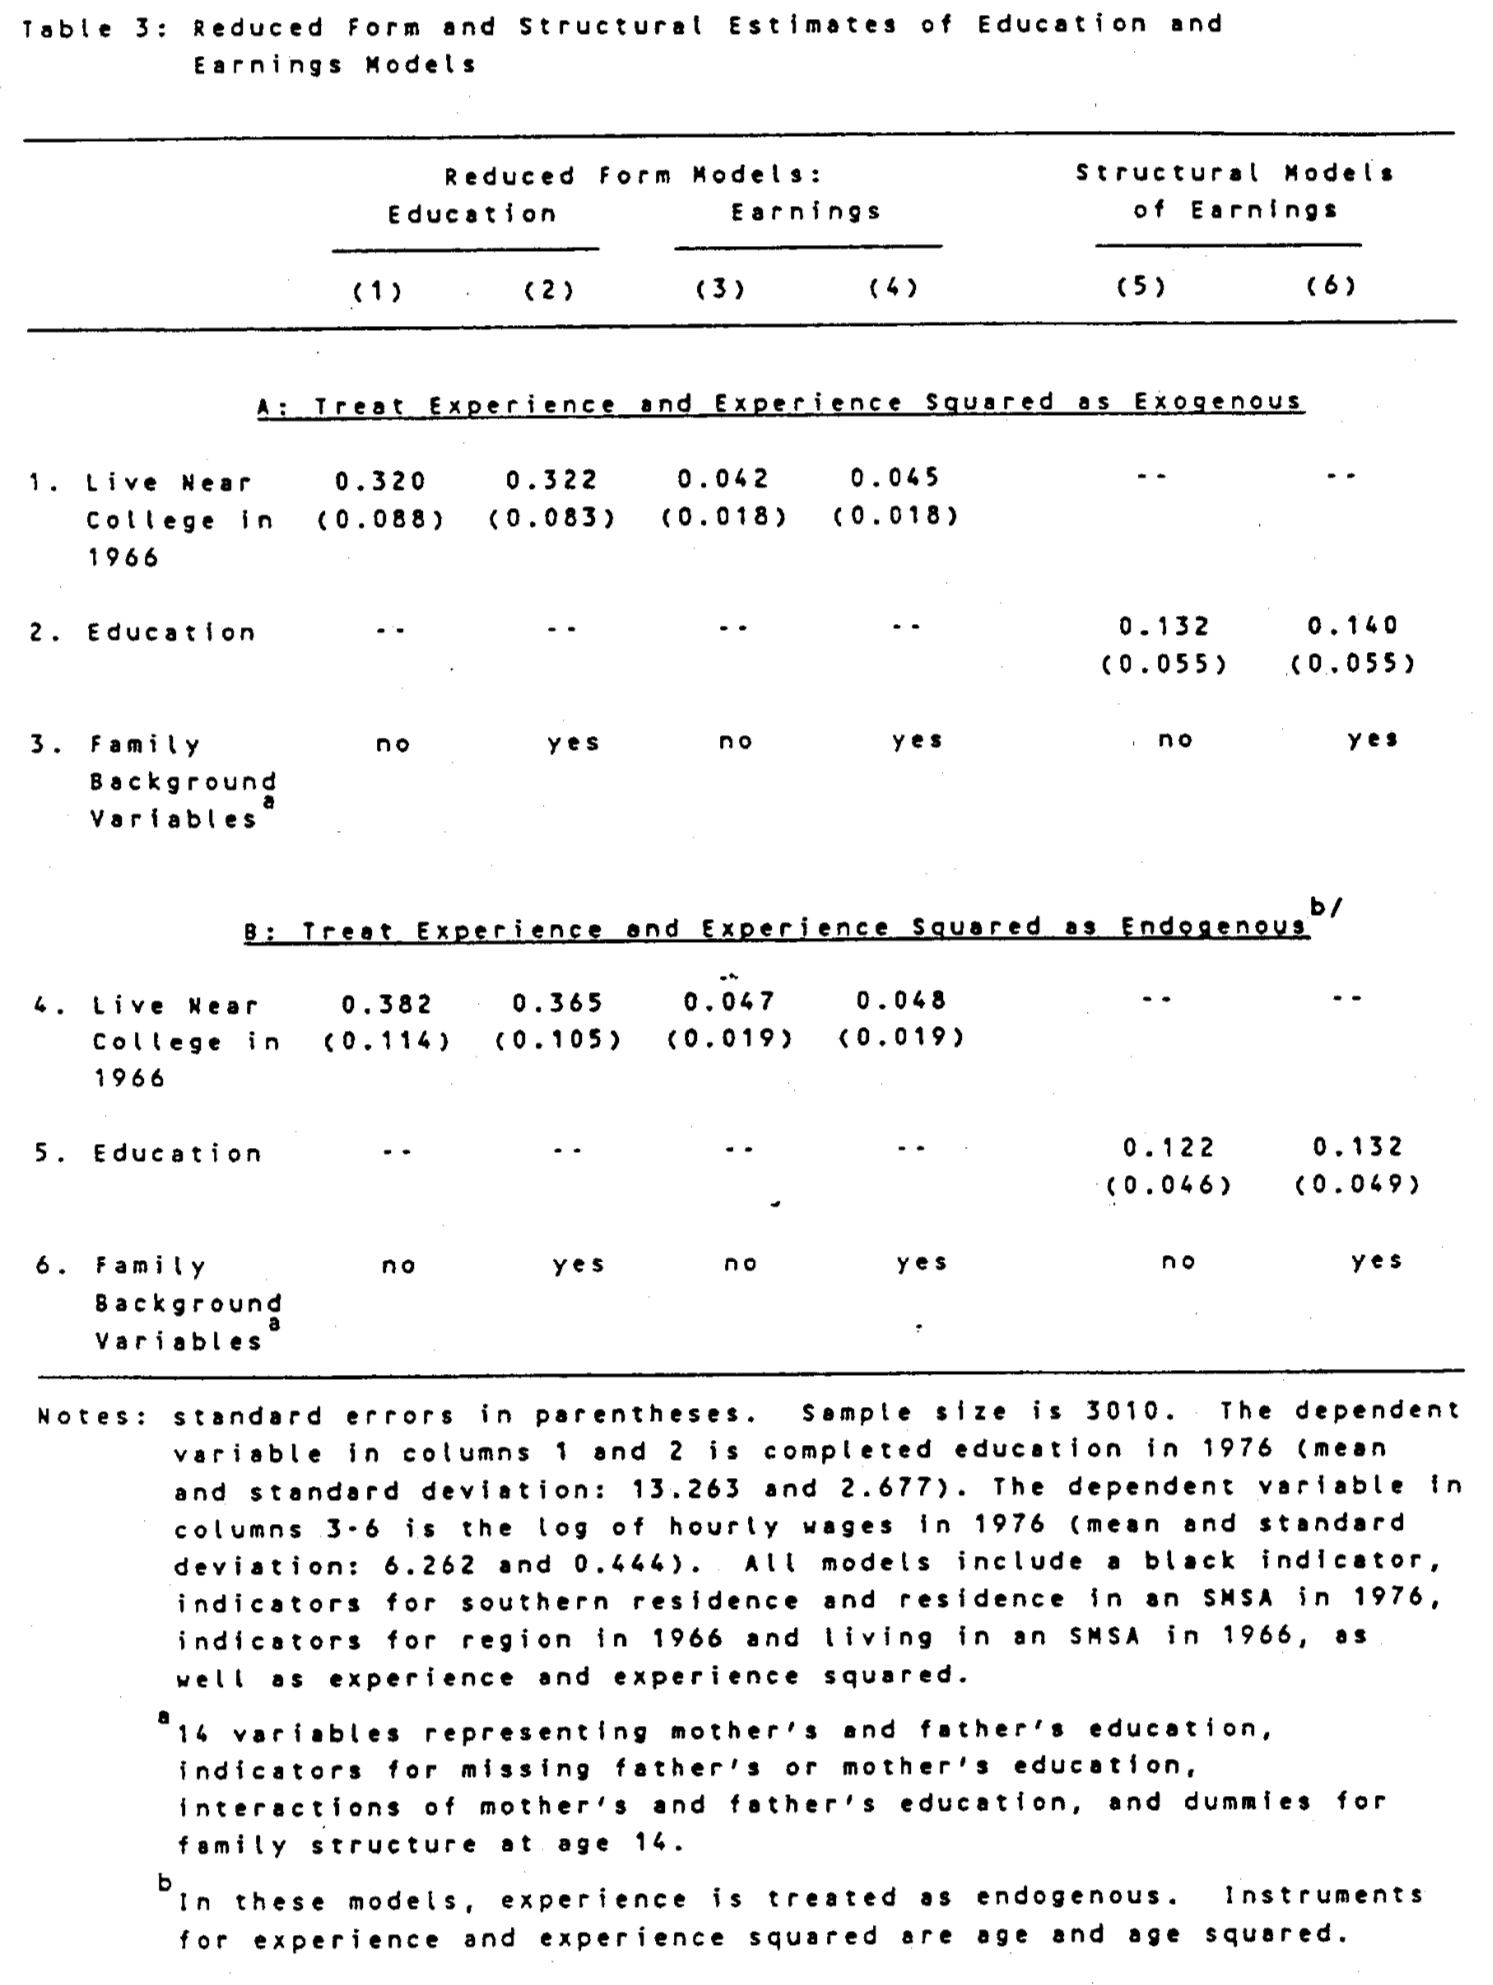
\includegraphics[scale=0.23]{table3.png}
\end{figure}\\
Table 2 shows the reduced from estimates for $educ$ containing all explanatory variables from part a and the dummy variable $nearc4.$ Our coefficient of interest is on $nearc4$ which is a dummy variable for someone living near a 4-year college. The estimates show that $educ$ and $nearc4$ are correlated with coefficient of 0.320 with a standard error of 0.0088. The result is statistically very significant. Thus the variable $nearc4$ satisfy the relevance condition for a good IV. Comparing with the result in Card (1995) as shown in Figure \ref{Fig3.2}, the result that we get is the same as in Column (1).
\\
\begin{table}[htbp]\centering
\def\sym#1{\ifmmode^{#1}\else\(^{#1}\)\fi}
\caption{Regression results for (1) Problem 5.4.b. and (2) Problem 5.4.d}
\begin{tabular}{l*{2}{c}}
\toprule
                    &\multicolumn{1}{c}{(1)}         &\multicolumn{1}{c}{(2)}         \\
\midrule
age - educ - 6      &      -0.413\sym{***}&      -0.412\sym{***}\\
                    &     (0.034)         &     (0.034)         \\
\addlinespace
exper^2             &       0.001         &       0.001         \\
                    &     (0.002)         &     (0.002)         \\
\addlinespace
=1 if black         &      -0.936\sym{***}&      -0.945\sym{***}\\
                    &     (0.094)         &     (0.094)         \\
\addlinespace
=1 if in south, 1976&      -0.052         &      -0.042         \\
                    &     (0.135)         &     (0.136)         \\
\addlinespace
=1 in in SMSA, 1976 &       0.402\sym{***}&       0.401\sym{***}\\
                    &     (0.105)         &     (0.105)         \\
\addlinespace
regional dummy, 1966&      -0.210         &      -0.169         \\
                    &     (0.202)         &     (0.204)         \\
\addlinespace
reg662              &      -0.289\sym{**} &      -0.269\sym{*}  \\
                    &     (0.147)         &     (0.148)         \\
\addlinespace
reg663              &      -0.238\sym{*}  &      -0.190         \\
                    &     (0.143)         &     (0.146)         \\
\addlinespace
reg664              &      -0.093         &      -0.038         \\
                    &     (0.186)         &     (0.189)         \\
\addlinespace
reg665              &      -0.483\sym{**} &      -0.437\sym{**} \\
                    &     (0.188)         &     (0.190)         \\
\addlinespace
reg666              &      -0.513\sym{**} &      -0.502\sym{**} \\
                    &     (0.210)         &     (0.210)         \\
\addlinespace
reg667              &      -0.427\sym{**} &      -0.378\sym{*}  \\
                    &     (0.206)         &     (0.208)         \\
\addlinespace
reg668              &       0.314         &       0.382         \\
                    &     (0.242)         &     (0.245)         \\
\addlinespace
=1 if in SMSA, 1966 &       0.025         &       0.000         \\
                    &     (0.106)         &     (0.107)         \\
\addlinespace
=1 if near 4 yr college, 1966&       0.320\sym{***}&       0.321\sym{***}\\
                    &     (0.088)         &     (0.088)         \\
\addlinespace
=1 if near 2 yr college, 1966&                     &       0.123         \\
                    &                     &     (0.077)         \\
\addlinespace
Constant            &      16.849\sym{***}&      16.773\sym{***}\\
                    &     (0.211)         &     (0.216)         \\
\midrule
Observations        &        3010         &        3010         \\
\bottomrule
\multicolumn{3}{l}{\footnotesize Standard errors in parentheses}\\
\multicolumn{3}{l}{\footnotesize Data: CARD.DTA}\\
\multicolumn{3}{l}{\footnotesize Wooldridge (2011)}\\
\multicolumn{3}{l}{\footnotesize \sym{*} \(p<0.10\), \sym{**} \(p<0.05\), \sym{***} \(p<0.01\)}\\
\end{tabular}
\end{table}


\item[c.] Estimate the $\log(wage)$ equation by IV, using $nearc4$ as an instrument for $educ.$ Compare the 95 percent confidence interval for the return to education with that obtained from part a. (See also Table 3, Column (5) in Card (1995).)
\\ Answer:\\
Using IV
\begin{table}[htbp]\centering
\def\sym#1{\ifmmode^{#1}\else\(^{#1}\)\fi}
\caption{Regression result for Problem 5.4.c.}
\begin{tabular}{l*{1}{c}}
\toprule
                    &\multicolumn{1}{c}{(1)}         \\
\midrule
years of schooling, 1976&       0.132\sym{**} \\
                    &     (0.055)         \\
\addlinespace
age - educ - 6      &       0.108\sym{***}\\
                    &     (0.024)         \\
\addlinespace
exper^2             &      -0.002\sym{***}\\
                    &     (0.000)         \\
\addlinespace
=1 if black         &      -0.147\sym{***}\\
                    &     (0.054)         \\
\addlinespace
=1 if in south, 1976&      -0.145\sym{***}\\
                    &     (0.027)         \\
\addlinespace
=1 in in SMSA, 1976 &       0.112\sym{***}\\
                    &     (0.032)         \\
\addlinespace
regional dummy, 1966&      -0.108\sym{***}\\
                    &     (0.042)         \\
\addlinespace
reg662              &      -0.007         \\
                    &     (0.033)         \\
\addlinespace
reg663              &       0.040         \\
                    &     (0.032)         \\
\addlinespace
reg664              &      -0.058         \\
                    &     (0.038)         \\
\addlinespace
reg665              &       0.038         \\
                    &     (0.047)         \\
\addlinespace
reg666              &       0.055         \\
                    &     (0.053)         \\
\addlinespace
reg667              &       0.027         \\
                    &     (0.049)         \\
\addlinespace
reg668              &      -0.191\sym{***}\\
                    &     (0.051)         \\
\addlinespace
=1 if in SMSA, 1966 &       0.019         \\
                    &     (0.022)         \\
\addlinespace
Constant            &       3.774\sym{***}\\
                    &     (0.935)         \\
\midrule
Observations        &        3010         \\
\bottomrule
\multicolumn{2}{l}{\footnotesize Standard errors in parentheses}\\
\multicolumn{2}{l}{\footnotesize Data: CARD.DTA}\\
\multicolumn{2}{l}{\footnotesize Wooldridge (2011)}\\
\multicolumn{2}{l}{\footnotesize \sym{*} \(p<0.10\), \sym{**} \(p<0.05\), \sym{***} \(p<0.01\)}\\
\end{tabular}
\end{table}



\item[d.] Now use $nearc2$ along with $nearc4$ as instruments for $educ$. First estimate the reduced form for $educ$, and comment on whether $nearc4$ is more strongly related to $educ$. How do the 2SLS estimates compare with the earlier estimates?
\\ Answer:\\

\item[e.] For as subset of the men in the sample, IQ score is available. Regress $iq$ on $nearc4.$ Is IQ score uncorrelated with $nearc4$?
\\ Answer:\\

\item[f.] Now regress $iq$ on $nearc4$ along with $smsa66, reg661, reg662,$ and $reg669.$ Are $iq$ and $nearc4$ partially correlated? What do you conclude about the importance of controlling for the 1966 location and regional dummies in the $\log(wage)$ equation when using $nearc4$ as an IV for $educ$?
\\ Answer:\\

\end{enumerate}


\subsection*{Problem 5.7}
Consider model (5.45) where $v$ has zero mean and is uncorrelated with $x_1,\ldots,x_K$ and $q$. The unobservable $q$ is thought to be correlated with at least some of the $x_j$. Assume without loss of generality that $\E(q)=0.$\\
You have a single indicator of $q$, written as $q_1=\delta_1q+a_1,\delta_1\neq 0,$ where $a_1$ has zero mean and is uncorrelated with each of $x_j,q$ and $v$. In addition, $z_1,z_2,\ldots,z_M$ is a set of variables that are (1) redundant in the structural equation (5.45) and (2) uncorrelated with $a_1.$
\begin{enumerate}
\item[a.] Suggest an IV method for consistently estimating the $\beta_j.$ Be sure to discuss what is needed for identification.
\\ Answer:\\

\item[b.] If equation (5.45) is a $\log(wage)$ equation, $q$ is ability, $q_1$ is IQ or some other test score, and $z_1,\ldots,z_M$ are family of variables, such as parents' education and number of siblings, describe the economic assumption needed for consistency of the IV procedure in part a.
\\ Answer:\\

\item[c.] Carry out this procedure using the data in NLS80.RAW. Include among the explanatory variables $exper, tenure,educ,married,south,urban,$ and $black$. First use $IQ$ as $q_1$ and then $KWW$. Include in the $z_h$ the variables $meduc,feduc,$ and $sibs.$ Discuss the results.
\\ Answer:\\
\end{enumerate}

\subsection*{Problem 5.11}
A model with a single endogenous explanatory variable can be written as
\[y_1=\textbf{z}_1\pmb{\delta}_1+\alpha_1y_2+u_1, \ \ \ \E(\textbf{z}'u_1)=0,\]
where $\textbf{z}=(\textbf{z}_1,\textbf{z}_2)$. Consider the following two-step method, intended to mimic 2SLS:
\begin{enumerate}
    \item[a.] Regress $y_2$ on $\textbf{z}_2$, and obtain the fitted values, $\Tilde{y}_2$. (That is. $\textbf{z}_1$ is omitted from the first-stage regression.)
    \item[b.] Regress $y_1$ on $\textbf{Z}_1, \Tilde{y}_2$ to obtain $\Tilde{\pmb{\delta}}_1$ and $\Tilde{\alpha}_1$. 
\end{enumerate}
Show that $\Tilde{\pmb{\delta}}_1$ and $\Tilde{\alpha}_1$ are generally inconsistent. When would $\Tilde{\pmb{\delta}}_1$ and $\Tilde{\alpha}_1$ be consistent? (Hint: Let $y_2^0$ be the population linear projection of $y_2$ on $\textbf{z}_2$, and let $a_2$ be the projection error: $y_2^0=\textbf{z}_2\pmb{\lambda}_2+a_2, \E(\textbf{z}_2'a_2)=\textbf{0}$. For simplicity, pretend that $\pmb{\lambda}_2$ is known rather than estimted; that is, assume that $\Tilde{y}_2$ is actually $y_2^0.$ Then, write:
\[y_1=\textbf{z}_1\pmb{\delta}_1+\alpha_1y_2^0+\alpha_1a_2+u_1\]
and check whether the composite error $\alpha_1a_2+u_1$ is uncorrelated with the explanatory variables.)
\\ Answer:\\



\subsection*{Problem 5.13}
Consider the simple regression model
\[y=\beta_1+\beta_1x+u\]
and let $z$ be a \textit{binary} instrumental variable for $x.$ 
\begin{enumerate}
\item[a.] Show that the IV estimator $\hat{\beta}_1$ can be written as
\[\hat{\beta}_1=(\bar{y}_1-\bar{y}_0)/(\bar{x}_1-\bar{x}_0),\]
where $\bar(y)_0$ and $\bar(x)_0$ are the sample averages of $y_i$ and $x_i$ over the part of the sample with $z_i=0$, $\bar(y)_1$ and $\bar(x)_1$ are the sample averages of $y_i$ and $x_i$ over the part of the sample with $z_i=1.$ This estimator, knows as a \textbf{grouping estimator}, was first suggested by Wald (1940).
\\ Answer:\\

\item[b.] What is the interpretation of $\hat{\beta}_1$ if $x$ is also binary, for example, representing participation in a social program?
\\ Answer:\\
\end{enumerate}

\section*{Chapter 6}
\subsection*{Problem 6.3}
Consider a model for individual data to test whether nutrition affects productivity (in a developing country):
\begin{align}
    \log(produc)=\delta_0+\delta_1exper+\delta_2exper^2+\delta_3educ+\alpha_1calories+\alpha_2protein+u_1, \tag{(6.57)} \label{(6.57)}
\end{align}
where $produc$ is some measure of worker productivity, $calories$ is calorie intake per day, and $protein$ is a measure of protein intake per day. Assume here that $exper,exper^2,$ and $educ$ are all exogenous. The variables $calories$ and $protein$ are possibly correlated with $u_1$ (See Strauss and Thomas (1995) for discussion). Possible instrumental variables for $calories$ and $protein$ are regional prices of various goods, such as grains, meats, breads, dairy products, and so on.
\begin{enumerate}
\item[a.] Under what circumstances do prices make good IVs for $calories$ and $protein$? What if prices reflect quality of food?
\\ Answer: \\

\item[b.] How many prices are needed to identify equation \eqref{(6.57)}?
\\ Answer: \\

\item[c.] Suppose we have $M$ prices, $p_1,\ldots,p_M.$ Explain how to test the null hypothesis that $calories$ and $protein$ are exogenous in equation \eqref{(6.57)}?
\\ Answer: \\
\end{enumerate}\\ 


\subsection*{Problem 6.7}
For this problem use the data in HPRICE.RAW, which is a subset of the data used by Kiel and McClain (1995). The file contains housing prices and characteristics for two years, 1978 and 1981, for homes sold in North Andover, Massachusetts. In 1981, construction on a garbage incinerator began. Rumors about the incinerator being built were circulating in 1979, and it is for this reason that 1978 is used as the base year. By 1981 it was very clear that the incinerator would be operating soon.
\begin{enumerate}
\item[a.] Using the 1981 cross section, estimate a bivariate, constant elasticity model relating housing price to distance from the incinerator. Is this regression appropriate for determining the causal effects of incinerator on housing prices? Explain.
\\ Answer:\\
\begin{table}[htbp]\centering
\def\sym#1{\ifmmode^{#1}\else\(^{#1}\)\fi}
\caption{Regression result for Problem 6.7.a.}
\begin{tabular}{l*{1}{c}}
\toprule
                    &\multicolumn{1}{c}{(1)}         \\
\midrule
log(dist)           &       0.365\sym{***}\\
                    &     (0.066)         \\
\addlinespace
Constant            &       8.047\sym{***}\\
                    &     (0.646)         \\
\midrule
Observations        &         142         \\
\bottomrule
\multicolumn{2}{l}{\footnotesize Standard errors in parentheses}\\
\multicolumn{2}{l}{\footnotesize Data: HPRICE.DTA}\\
\multicolumn{2}{l}{\footnotesize Wooldridge (2011)}\\
\multicolumn{2}{l}{\footnotesize \sym{*} \(p<0.10\), \sym{**} \(p<0.05\), \sym{***} \(p<0.01\)}\\
\end{tabular}
\end{table}


\item[b.] Pooling the two years of data, consider the model
\[\log(price)=\delta_0+\delta_1y81_\delta_2\log(dist)+\delta_3y81\cdot \log(dist)+u.\]
If the incinerator has a negative effect on housing prices for homes closer to the incinerator, what sign is $\delta_3$? Estimate this model and test the null hypothesis that the incinerator had no effect on housing prices. 
\\ Answer:\\
\begin{table}[htbp]\centering
\def\sym#1{\ifmmode^{#1}\else\(^{#1}\)\fi}
\caption{Regression results: (1) Problem 6.7.b. and (2) 6.7.c}
\begin{tabular}{l*{2}{c}}
\toprule
                    &\multicolumn{1}{c}{(1)}         &\multicolumn{1}{c}{(2)}         \\
\midrule
y81                 &      -0.011         &      -0.230         \\
                    &     (0.805)         &     (0.488)         \\
\addlinespace
log(dist)           &       0.317\sym{***}&       0.087\sym{*}  \\
                    &     (0.052)         &     (0.052)         \\
\addlinespace
y81 x log(dist)     &       0.048         &       0.062         \\
                    &     (0.082)         &     (0.050)         \\
\addlinespace
log(intst)          &                     &       0.963\sym{***}\\
                    &                     &     (0.326)         \\
\addlinespace
lintst^2            &                     &      -0.059\sym{***}\\
                    &                     &     (0.019)         \\
\addlinespace
log(area)           &                     &       0.355\sym{***}\\
                    &                     &     (0.051)         \\
\addlinespace
log(land)           &                     &       0.110\sym{***}\\
                    &                     &     (0.025)         \\
\addlinespace
age of house        &                     &      -0.007\sym{***}\\
                    &                     &     (0.001)         \\
\addlinespace
age^2               &                     &       0.000\sym{***}\\
                    &                     &     (0.000)         \\
\addlinespace
# rooms in house    &                     &       0.047\sym{***}\\
                    &                     &     (0.017)         \\
\addlinespace
# bathrooms         &                     &       0.096\sym{***}\\
                    &                     &     (0.027)         \\
\addlinespace
Constant            &       8.058\sym{***}&       2.306         \\
                    &     (0.508)         &     (1.774)         \\
\midrule
Observations        &         321         &         321         \\
\bottomrule
\multicolumn{3}{l}{\footnotesize Standard errors in parentheses}\\
\multicolumn{3}{l}{\footnotesize Data: HPRICE.DTA}\\
\multicolumn{3}{l}{\footnotesize Wooldridge (2011)}\\
\multicolumn{3}{l}{\footnotesize \sym{*} \(p<0.10\), \sym{**} \(p<0.05\), \sym{***} \(p<0.01\)}\\
\end{tabular}
\end{table}


\item[c.] Add the variables $\log(intst),[\log(intst)]^2,\log(area),\log(land),age,age^2,rooms,baths$ to the model in part b, and test for an incinerator effect. What do you conclude?
\\ Answer:\\

\end{enumerate}

\section*{Non-textbook Problem}
Derive the variance of the IV estimator for the case of heteroskedasticity.
\\ Answer:\\

\end{document}